\chapter{Methoden}

\section{Python-Interface f"ur MCTDH}
\label{sec:PyInterface}

Es wurden einige Klassen aus dem MCTDH-C++ Code mit Cython importiert, die f"ur das Einlesen der baumf"ormig strukturierten MCTDH-Basis zust"andig sind.
Diese Klassen und deren Methoden sind in Abbildung \ref{fig:uml_Cython} dargestellt. 

\begin{figure}
    \centering
    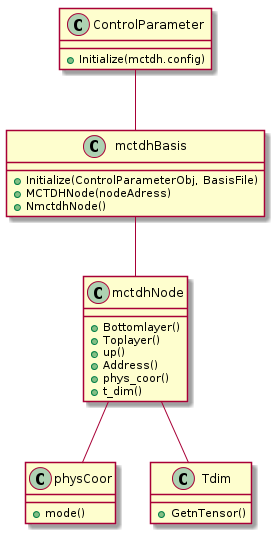
\includegraphics[scale=0.6]{figures/sequenceDiagram}
    \caption{Alle Klassen, die in Cython erstellt wurden, sind mit einem ,,C'' gekennzeichnet. Die jeweiligen Klassenmethoden sind mit einem
    gr"unen Punkt gekennzeichnet.}\label{fig:uml_Cython}
\end{figure}


Jedes Rechteck mit einem umkreisten \textit{C} gibt den Name der in Python importierten Klasse an. 
\textit{ControlParameter} und \textit{mctdhBasis} sind die Klassen, die die Konfigurations- und Basisdatei mithilfe der Methode
\textit{Initialize} einlie"st. \textit{NmctdhNode} gibt die Anzahl der Knoten der baumf"ormigen Basis.
Mithilfe der Methode \textit{MCTDHNode} werden Objekte erzeugt, die stellvertretend f"ur eine Knoten des Baums stehen
und der Klasse \textit{mctdhNode} zu zuordnen sind. Das Argument dieser Methode ist ganzzahlig und entspricht der internen Knotennummerierung.
Zu den Knoten k"onnen Information, ob der Knoten den obersten Knoten darstellt oder zu den untersten Knoten geh"ohrt, abgefragt werden.
\textit{Toplayer} und \textit{Bottomlayer} geben Booleans als R"uckgebewert wieder und \textit{adress} gibt die jeweilige Knotennummerierung 
wieder. Mit \textit{up} wird der Knoten in den n"achsth"oheren Knoten "uberf"uhrt.
Die Knotenobjekte k"onnen in die Klassen \textit{physCoor} und \textit{Tdim} "uberf"uhrt werden. Mit diesen Klassen k"onnen
die Schwingungsmoden, der untersten Knoten, sowie die SPFs der jeweiligen Knoten ermittelt werden. 





\section{Graphische Benutzeroberfl"ache f"ur MCTDH}

 Die graphisch Benutzeroberfl"ache (GUI) f"ur MCTDH-Rechnungen wurde in Python und Qt implementiert.
 Der Zugriff auf die Qt-Bibliothek erfolgt "uber die Python-Bibliothek PyQt4. 
 PyQt4 umfasst zehn Python-Module, die zusammen ungef"ahr 400 Klassen und 6000 Methoden und Funktionen enthalten. \cite{PyQt}

 \begin{figure}
    \centering
    \vspace*{-0.5cm}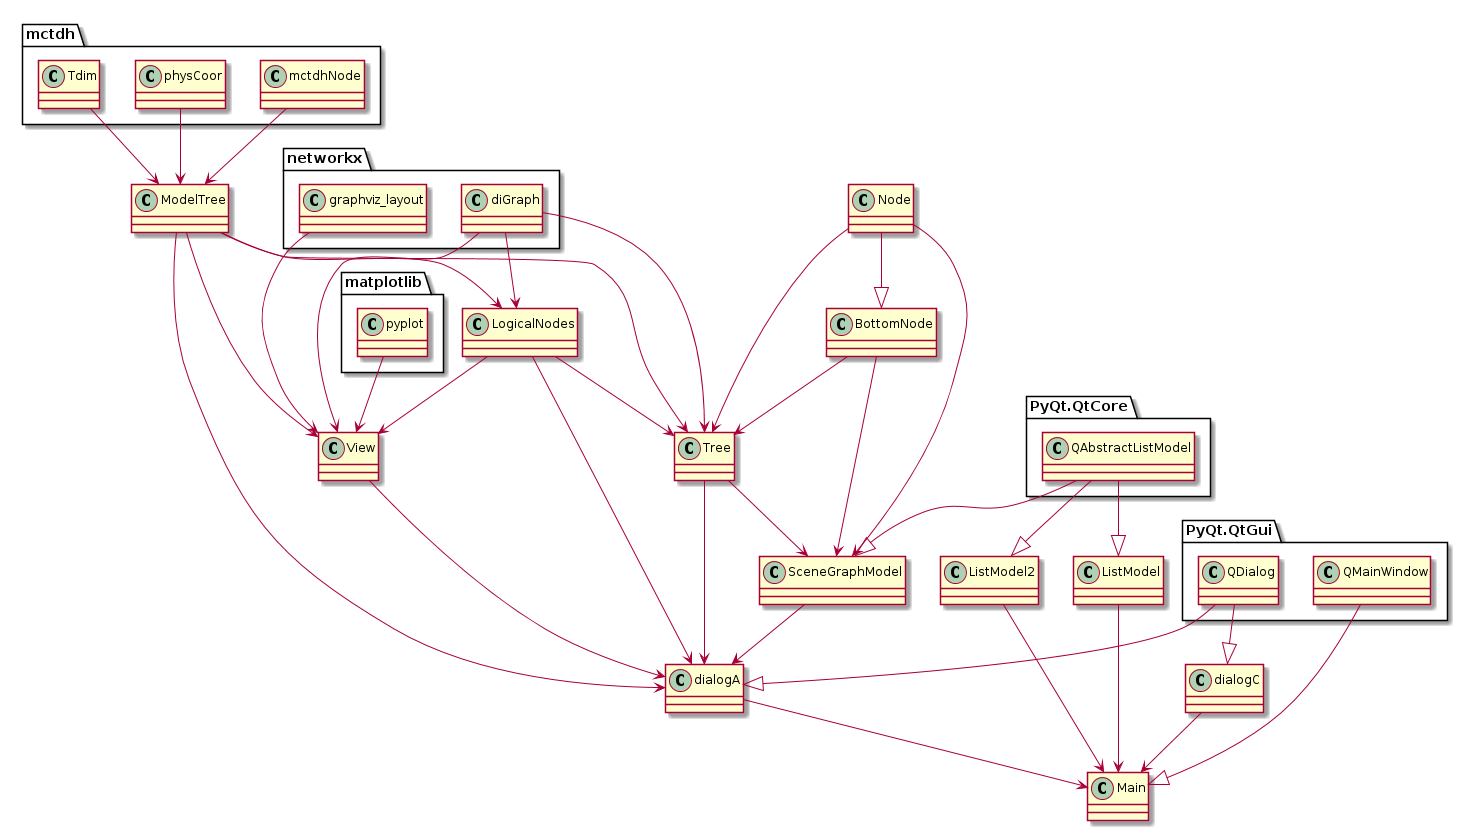
\includegraphics[width=\textwidth, angle=90, scale=1.4]{figures/umlPyQt}
    \caption{Klassendiagram der MCTDH-GUI. Eine Beschreibung des Diagramms
     findet sich im Text wieder.}\label{fig:uml_PyQt}
\end{figure}

In Abbildung \ref{fig:uml_PyQt} sind die wichtigen Klasse aufgef"uhrt, die f"ur die Implementierung der GUI verwendet wurden. 
Die Klassen, die in Rechtecken zusammengefasst wurden, entstammen aus Python-Modulen, deren Namen links "uber den Rechtecken angegeben sind.
Bei den Modulen handelt es sich um die PyQt4-Module \textit{QtCore} und \textit{QtGui}. F"ur die graphisch Darstellung der MCTDH-Baumdiagramme
wurden die Module \textit{matplotlib} und \textit{networkx} verwendet. Die Klassen, die in Abschnitt \ref{sec:PyInterface} vorgestellt wurden,
sind im Modul \textit{mctdh} enthalten. Die Pfeile mit den ausgef"ullten Pfeilk"opfen  f"uhren von Klassen, die in anderen Klassen verwendet werden,
auf die der Pfeil zeigt.
Auf die Klassen, die durch Vererbung erstellt wurden, zeigen rot umrandete Pfeilspitzen. Beispielswei"se f"uhren diese Pfeile von allen angegeben PyQt-Klassen
, von denen geerbt wird.
Sowohl von \textit{QDialog} als auch \textit{QMainWindow} werden durch Vererbung Unterklassen generiert: \textit{dialogA, dialogc} und \textit{Main}. 
Die beiden Klassen\textit{QDialog} und \textit{QMainWindow} stammen von \textit{QWidget} ab. \textit{QWidget}, \textit{QDialog} und \textit{QMainWindow}
sind Steuerungselement, mit denen der Benutzer durch die Tastatur und Maus interagieren kann, die sich in ihren Merkmalen unterscheiden: So ist
schlie"st das Dialogfenster, wenn der Benutzer den X-Knopf klickt. Wenn ein Widget geschlossen wird, ist es lediglich versteckt. \cite{PyQt}
Qt enth"alt Klassen, mit denen beliebig viele Elemente dargestellt werden k"onnen. Diesen Klassen liegt eine Model/View-Aufbau zugrunde,
 der das Datenmodel von der Darstellung der Daten trennt. 
Ein Datenmodel ist die Klasse \textit{QAbstractListModel}, in die die Daten eingelesen, bearbeitet und gel"oscht werden k"onnen.
Die Daten k"onnen wiederum in den Klassen \textit{QListView} und \textit{QTreeView} dargestellt werden. 
Die Trennung zwischen dem Datenmodel und der graphischen Darstellung der Daten beruht auf dem Model-View-Controller (MVC) Paradigma.\cite{Qt}  

  




   
